% vim: set tw=78 sts=2 sw=2 ts=8 aw et ai:
\documentclass[12pt]{article}

\usepackage[paper=a4paper, top=2cm, bottom=3cm, left=2.5cm, right=2.5cm]{geometry}

\usepackage{ucs}
\usepackage[utf8x]{inputenc}
\usepackage[english]{babel}
%\usepackage{hyperref}	  % use \url{http://$URL} or \href{http://$URL}{Name}
\usepackage{underscore}	  % underscores need not be escaped
\usepackage{subfigure}
\usepackage{verbatim}
\usepackage{float}
\usepackage{booktabs}     % professional tables
\usepackage{parskip}

% Support for including graphics
\usepackage{graphicx}
\DeclareGraphicsExtensions{.pdf,.png,.jpg}

\title{Securing IoT Networks}

\author{
Student Andrei Vlădescu \\  Professor Dr. Ion Bica \\
Faculty of Automatic Control and Computers\\
University POLITEHNICA of Bucharest\\
\emph{vladescu.andrei@techbattlefield.ro}}

\date{\today}

\begin{document}

\maketitle

\begin{abstract}
% vim: set tw=78 sts=2 sw=2 ts=8 aw et ai:
This study investigates the efficacy of Moving Target Defense (MTD) strategies in bolstering the security of Internet of Things (IoT) networks. With the escalating integration of diverse and resource-constrained IoT devices into critical infrastructures, traditional security measures prove insufficient against evolving threats. Our research assesses MTD techniques, such as dynamic network reconfiguration and software diversity, demonstrating their effectiveness in enhancing resistance to both known and zero-day attacks. The adaptive nature of MTD mechanisms ensures continuous adjustments, providing robust protection for systems, such as IoT devices. These findings provide insights for developers, security engineers, and researchers in search of adaptive solutions to safeguard IoT ecosystems from the ever-changing threat landscape.
\end{abstract}

\section{Introduction}
\label{sec:introduction}
The surge in Internet of Things (IoT) devices has transformed our daily lives, linking everything from home gadgets to industrial equipment. According to \cite{number_of_iot_devices}, the number of these IoT devices will almost double from 2023 to 2030, to a number of aproximately 30 billion devices. While this connectivity brings convenience, it also raises important security concerns. IoT devices, now included inside many homes and facilities, require a focus on security to address potential risks. This paper aims to explore the security aspects of IoT devices, emphasizing the need for practical measures. One such important security measure is called Moving Target Defense (MTD).\\
MTD methodology typically falls under the category of proactive security measures, as it aims to evade security threats, thus making it more difficult for an attacker to deliver a malicious payload.\\
The objective of this paper is to provide a overview of the existing body of knowledge. By scrutinizing contemporary literature, research papers, and case studies, this document aims to focus on the current state of MTD in IoT, elucidating the key principles, challenges, and potential strongpoints for future exploration.

\section{MTD Strategy applied in IoT}
\label{sec:mtd_strategy}
MTD can best be described as the classical game of "shell game" \cite{cho2019proactive}, in which a stone is hidden under three cups or shells, and the gambler tries to guess the location of the stone, after they were shuffled.\\
In the words of \cite{mtd_vol1}, moving target defenses have been proposed as a way to make it much more difficult for an attacker to exploit a vulnerable system by changing aspects of that system to present attackers with a varying attack surface. The goal of a diverse defense is to make the attack target unpredictable, making it more difficult to deliver a malicious packet. Such strategies are already in place in a computer, such as address space layout randomization (ASLR), instruction set randomization (ISR), honeypots (decoy nodes) or honeynets (decoy networks). As such, different parameters can be varied so that the attacker will either miss his target, or worse, hit a decoy target.\\
In the space of IoT, the targets are usually small nodes, with a low power consumption, sometimes in hard-to-reach locations. Some of these attacks, that aim to bring down nodes will catastrophically affect these devices, as they may be either something trivial as a light bulb, or something that belongs to a city's infrastructure \cite{iot_electric_grid}. These MTD methodologies must be effective, in relation to a certain attack, must not add much overhead, as IoT devices are computationally slow, and they will possibly consume more power only by adding a framework specifically for this defense mechanism.

\section{State-of-the-Art MTD Techniques}
\label{sec:soa_mtd}
In the works of \cite{mtd_techniques} it is argued that MTD can be classified into four big categories. This is not the only article that tackles MTD categorization, others have done so too, in \cite{mtd_review_of_defense_mechanisms} or \cite{mtd_other_classification_methods}, but \cite{mtd_techniques} draws a better distinction between MTD strategies.

\subsection{Software-based Diversification}
The first technique which is discussed is software-based diversification. Existing works achieve this technique by manipulating the programs or compilers to produce diveresification. Via software manipulation, the security can be enhanced by input rectification, since excision may limit the payload type. An implementation is SOAP \cite{soap_software_mtd_technique} a software for rectifying input based on constraints.\\ 
Compiler-generated diversity attains it's purpose by producing internally different program variants, but with the same functions. Such works are presented by \cite{mtd_vol1}, in Chapter 4: massive-scale software diversity (MSSD) and malt-variant execution environment (MVEE).

\subsection{Runtime-based Diversification}
Several defense techniques address attacks by introducing diversification into runtime environments. One such technique is address space layout randomization (ASLR) \cite{aslr_runtime_mtd_technique}. ASLR randomizes the processes' address space, so that the attacker cannot use hard-coded addresses of a reconnoitered function or variable. Another such defense mechanism is instruction set randomization (ISR) \cite{isr_runtime_mtd_technique}. ISR encodes machine code with a compile-time randomized key. At runtime, the instructions are deobfuscated, so that the program can go freely. As an attacker, hardcoding a machine-code instruction will lead  to the illegal instruction error, and the program will terminate, thus protecting it. 

\subsection{Communication Diversification}
Communication diversification techniques safeguard systems from network-related attacks by concealing internal information and communication protocols. One such implementation of this scheme is the mutable networks  (MUTE) architecture, as it's presented in chapter nine of \cite{mtd_vol1}. MUTE enables networks to change their configurations such as IP address and routes randomly and dynamically while preserving the requirements and integrity of network operation. Adding decoys, the attacker can be tricked into fingerprinting the nodes on the network with wrong information.

\subsection{Dynamic Platform Techniques}
Dynamic platform techniques (DPT)\cite{mtd_other_classification_methods} change platform properties to stop attacking processes, like temporal changes (virtual machine rotation) or diversity (multiple variants of execution). Intersecting dynamic techniques at compiler-level are not discussed in this subsection, as they have been already covered. Talent \cite{talent_mtd_dynamic_technique} is a migration-based technique that leverages OS-level virtualization to create a virtual execution envirnoment for migrating a running application across different platoforms and preserving the state of the execution. DPT implementations can also be achieved by switching between different types of servers (e.g. Flask or Apache),  as proposed in \cite{web_servers_mtd_dynamic_technique}.

\subsection{Security Model}
The security model of identify, protect, detect, respond and recover (IPDRR) \cite{mtd_security_model_framework} is a traditional security model, that consists of standards, guidelinesand best practices. 

\begin{figure}[htbp]
  \centering
  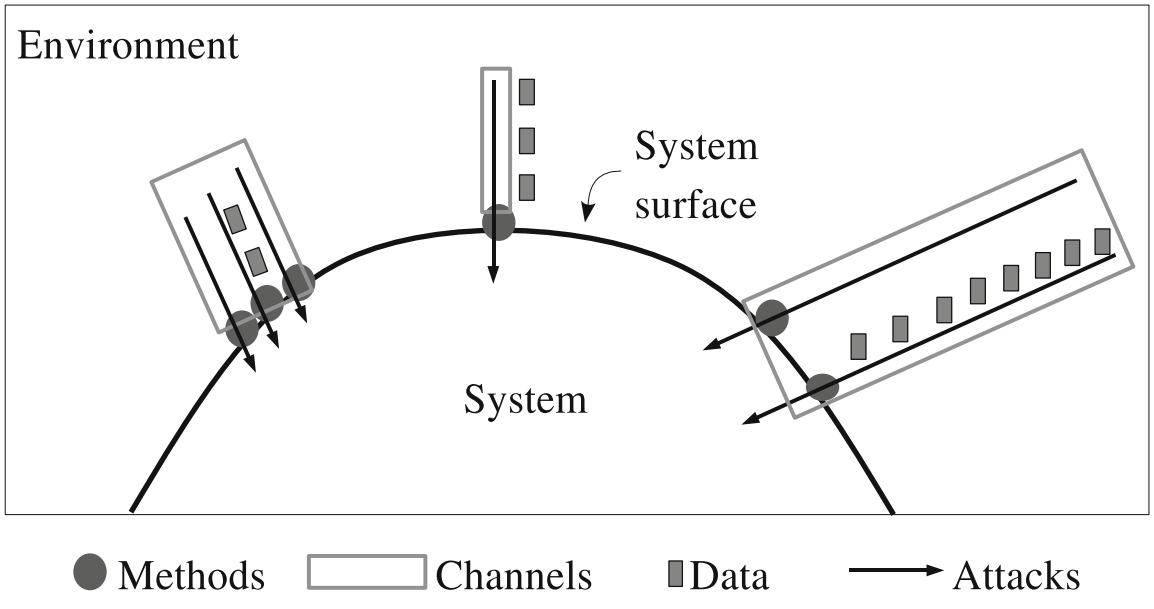
\includegraphics[width=0.7\linewidth]{img/system_attack_surface.png}
  \caption{System's Attack Surface\cite{mtd_vol1}}
  \label{fig:system_attack_surface}
\end{figure}

While the framework may be used in MTD, we can derive a better model for this usecase. New security models have been developed and measured \cite{mtd_security_model} \cite{mtd_book2} \cite{mtd_security_model_metric}. To have a better grasp of the problem encountered, an attack surface definition is in due. A system’s attack surface is the subset of the system’s resources that an attacker can use to attack the system. The taxonomy of the attack surface may be categorised into more smaller elements.

\subsubsection{Entry Points}
A system's entry points are methods, such as the system's API, that receive data items from the environment. For instance, a direct entry point, like a method receiving input from a user or reading a configuration file, can be invoked by a user or system in the environment, read from a persistent data item, or invoke another system's API. Indirect entry points receive data from direct entry points.

\subsubsection{Exit Points}
The system's exit points are methods, such as the one writing to a log file, that send data items to the environment. A direct exit point, like a method invoked by a user or system receiving data results, can write to a persistent data item or invoke another system's API with data items as input. An indirect exit point sends data to a direct exit point.

\subsubsection{Channels}
Systems have communication channels, like TCP/UDP sockets or RPC end points, which users or external systems use to interact. Attackers exploit these channels to connect to the system and invoke methods, adding another potential avenue for attacks.

\subsubsection{Untrusted Data Items}
An attacker utilizes persistent data items to either indirectly inject data into the system or receive data indirectly from it. Examples of persistent data items include files, cookies, database records, and registry entries. For instance, a system may read from a file after an attacker writes into it, or vice versa. Consequently, persistent data items serve as another vulnerability for potential attacks on a system.

\begin{figure}[htbp]
  \centering
  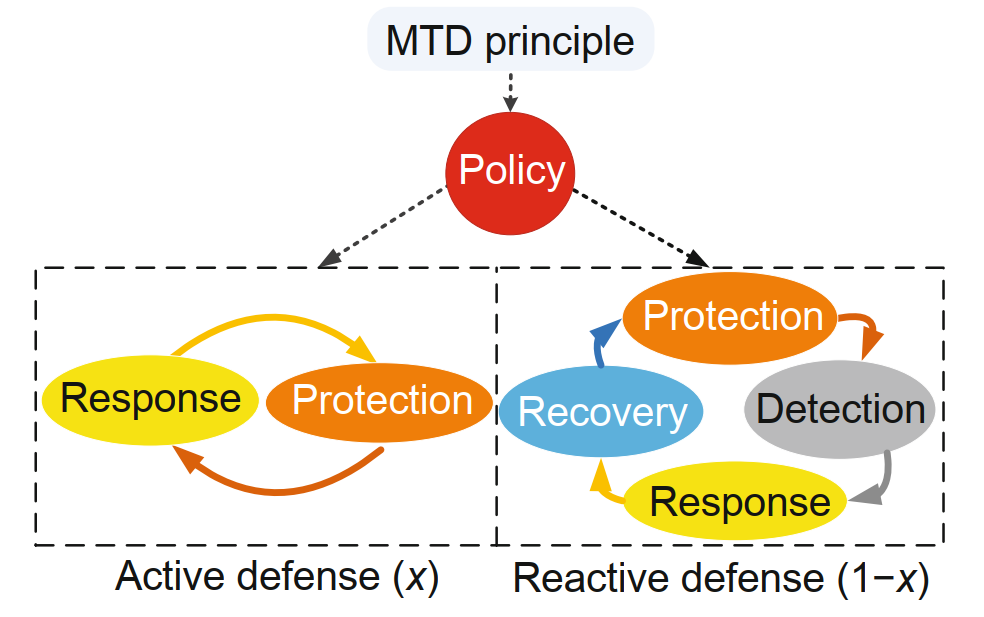
\includegraphics[width=0.7\linewidth]{img/mtd_new_ model.png}
  \caption{New Security Model for MTD\cite{mtd_security_model}}
  \label{fig:new_model}
\end{figure}


A new security model encompasses both active defense and reactive defense processes. In the active mode, defense operates independently of network status, periodically or irregularly shifting the attack surface. As a result, detection and recovery links are not required. In the reactive mode, the defense process is initiated by security alerts, aligning with the IPDRR model. x is the measurement of active defenses, and 1-x is the reactive defense measurement. A defense mechanism may employ a security system with different x, thus changing the dynamic.  


\section{Conclusion and Further Work}
\label{sec:conclusion}
In conclusion, this review highlights the critical significance of moving target defense in reinforcing the security posture of IoT devices. This examination of existing literature, case studies, and research findings aims to find a good balance for the problematic landscape of IoT security. By implementing these measures, the defense mechanisms act as a robust deterrent against malicious activities targeting the interconnected nature of IoT devices. Looking ahead, the identified gaps and limitations in current MTD strategies offer valuable insights for focused research initiatives. Given the dynamic and evolving nature of both IoT and cybersecurity, ongoing refinement of new security solutions for IoT is imperative.

\bibliographystyle{abbrv}
\bibliography{my-report}

\end{document}
